\section{It lives!}


\todo[inline]{Parece propaganda }
Translating the MDA framework into UFO led to a simple diagram with important information. Although simplistic, MDA has a lot of nuances. When addressed in a more complex modeling language this nuances need careful analysis to be correctly modeled. The diagram features in \autoref{fig:gamediagram} and its information detailed in sequence.

\begin{figure}[!h]
    \centering
    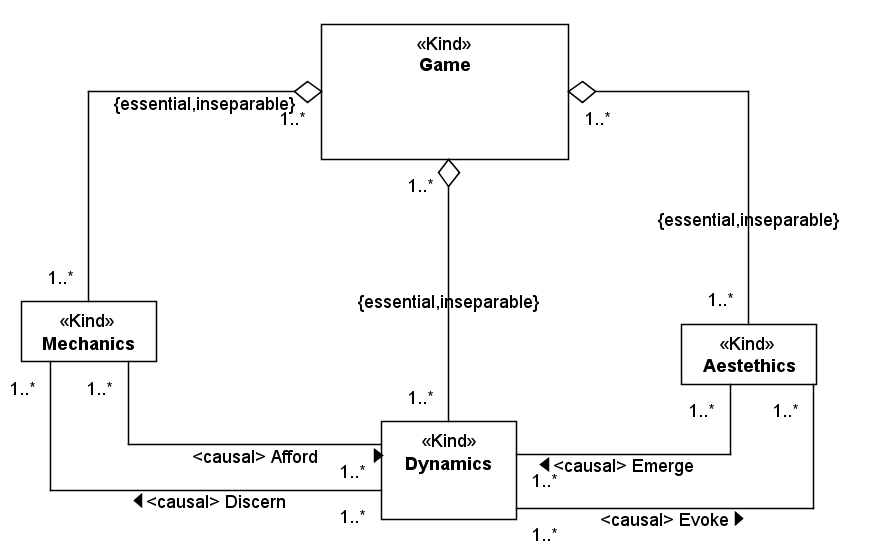
\includegraphics[scale=0.65]{Images/Model/Game.png}
    \caption{Game Diagram}
    \label{fig:gamediagram}
\end{figure}

This diagram illustrates the main idea of the MDA. The game is made of three different parts, mechanics, dynamics and aesthetics. They are inseparable and essential because a game must have all of them and they are intrinsic parts of games.

Addressing the designer and player different perspectives in MDA, the model includes the causal relationship between mechanics, dynamics and aesthetics. They were established in accordance to the discussion made in section 5.1.1.
